\documentclass[11pt]{article}\usepackage[margin=.7in]{geometry}\usepackage{graphicx,longtable,booktabs,amsmath}\setlength{\parindent}{0pt}\begin{document}\section*{250-episode return to A, B and C}
EXPLORATORY VALIDATION ONLY; no held-out tests -- PARTIAL RUN

PARTIAL REPORT: only the task groups listed below have been computed. B/C results are not claimed until their simulations finish. Three independent comparisons: A-B-C-D-return A, A-B-C-D-return B, and A-B-C-D-return C. The return simulator starts from the corresponding saved reference state, with frozen final weights. The repeated A-B-C-D prefix is reused from the saved checkpoints; it is not trained a second time on top of D. Original A validation metrics and models are reused exactly. For the new B/C comparisons, replay branches start from the saved ordinary checkpoint immediately after learning B/C and replay only that target through later tasks. Original ordinary checkpoints are reused as the matched no-replay controls. The 250 original episodes and splits are unchanged. No new teacher data are collected. No held-out test trajectories are opened. These additional validation comparisons are exploratory, not independent evidence from new test data. More cases or replay do not guarantee a win.

Original A replay candidates did not pass every new-task force-adaptation constraint. Their A retention curves are still shown, but are not relabelled as eligible final controllers. B/C eligibility and initial-task tracking quality are also reported. If the controller was inaccurate at learning, poor later tracking alone is not evidence of forgetting. A force-imitation gate is not itself a closed-loop angle-tracking measurement.
\section*{Architecture and continual-learning objective}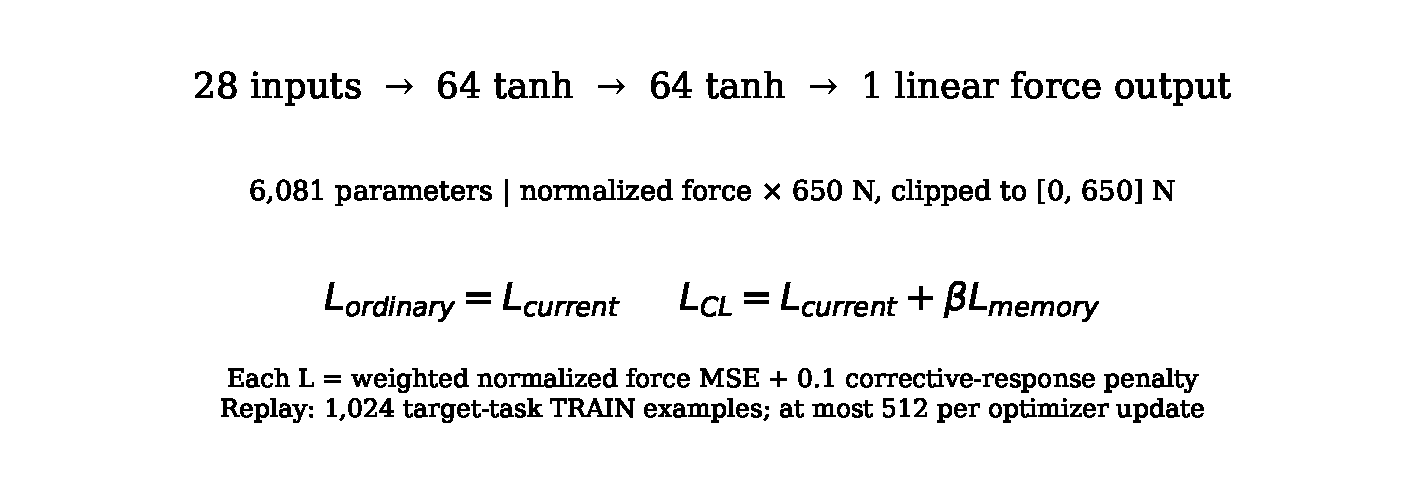
\includegraphics[width=\linewidth]{figures/architecture/network_and_cost.pdf}
\[L_{CL}=L_{cur}+\beta L_{mem},\quad L_{cur}=\frac{\sum_i w_i(\hat f_i-f_i)^2}{\sum_i w_i}+0.1P_{cur}.\]
Force targets are normalized by 650 N. The memory term uses the same weighted force MSE and response penalty on stored training examples. Startup weights are 25 in the first 0.25 s, 8 for the remainder of the first second, 1 otherwise; teacher-query rows have weight 6. The response penalty discourages encoded angle/velocity corrective slopes below 0.02 using centered finite differences of step 0.05. It uses at most 128 current or replay examples. Both branches use Adam, learning rate 0.001, batch size 2048, and 120 epochs per later task. A maximum of 512 old-task examples is replayed per update from a fixed memory of 1024 examples. This is target-specific episodic replay, not EWC.
\clearpage\section*{Validation table}\small\begin{longtable}{llrrrrr}\toprule Task & Model & Tried & Done & Fail & Pass & RMSE deg\\\midrule
A\_90 & learned & 6 & 6 & 0 & 6 & 0.0209\\
A\_90 & noCL & 6 & 6 & 0 & 0 & 4.9075\\
A\_90 & CL\_beta\_1 & 6 & 6 & 0 & 6 & 0.0466\\
A\_90 & CL\_beta\_4 & 6 & 6 & 0 & 6 & 0.0810\\
A\_90 & CL\_beta\_16 & 6 & 6 & 0 & 5 & 2.7639\\
B\_60 & learned & 6 & 6 & 0 & 6 & 0.0231\\
B\_60 & noCL & 6 & 5 & 1 & 2 & 3.5560\\
B\_60 & CL\_beta\_1 & 6 & 6 & 0 & 3 & 3.8154\\
\bottomrule\end{longtable}\normalsize
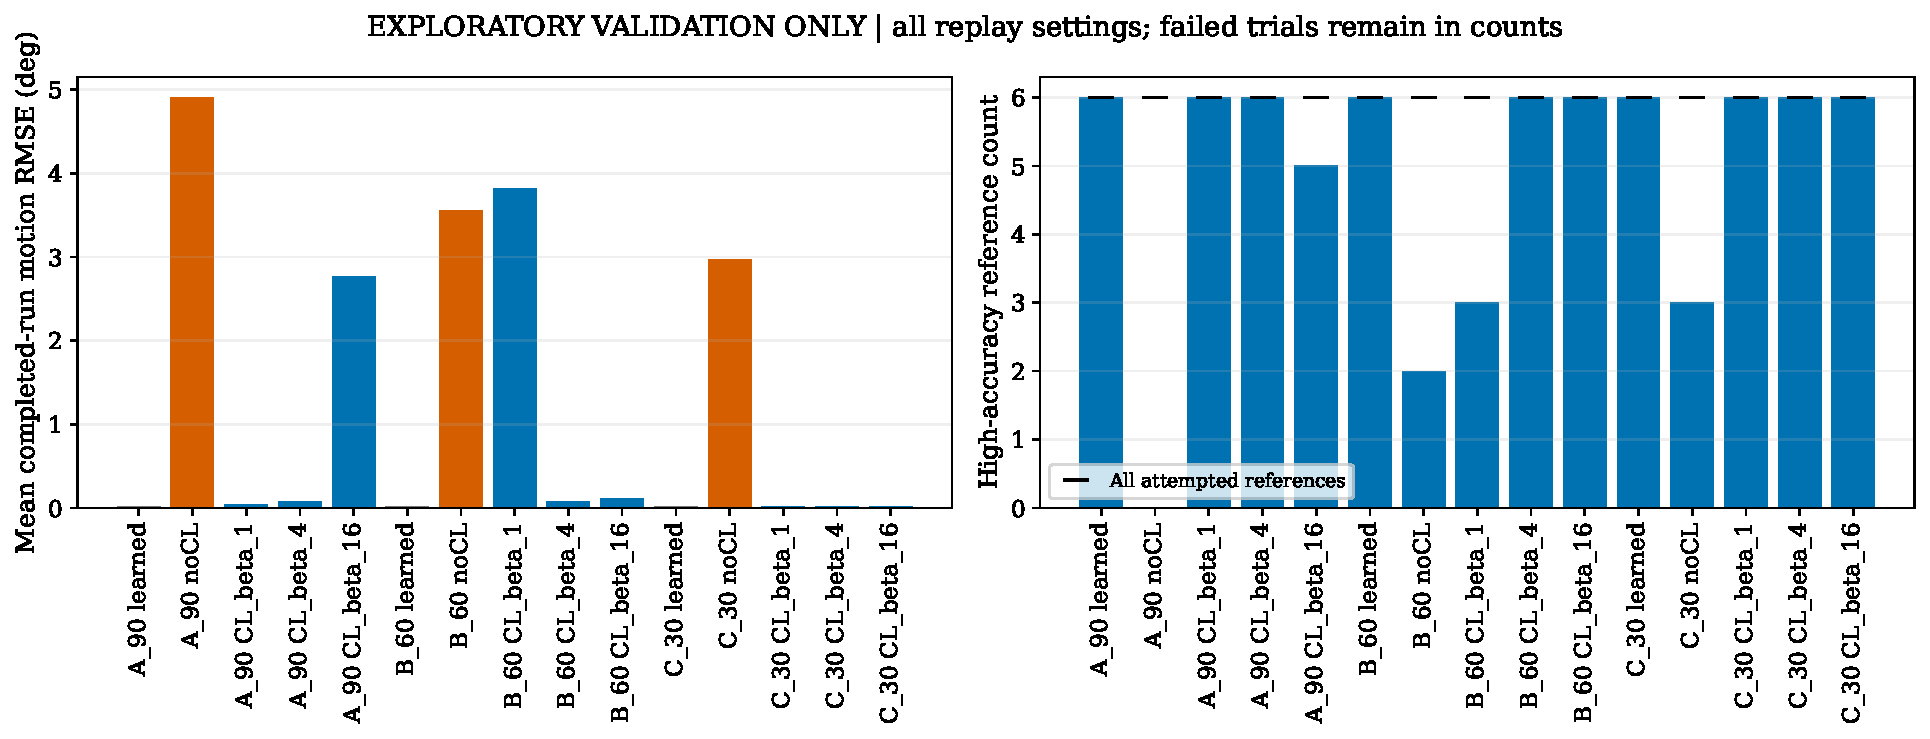
\includegraphics[width=\linewidth]{figures/summary/all_candidates.pdf}
\section*{Predeclared primary comparison: beta=1}
The first reference in sorted ID order is shown for each task, without choosing the easiest or largest improvement. The separate appendix includes all references and all replay weights.
\clearpage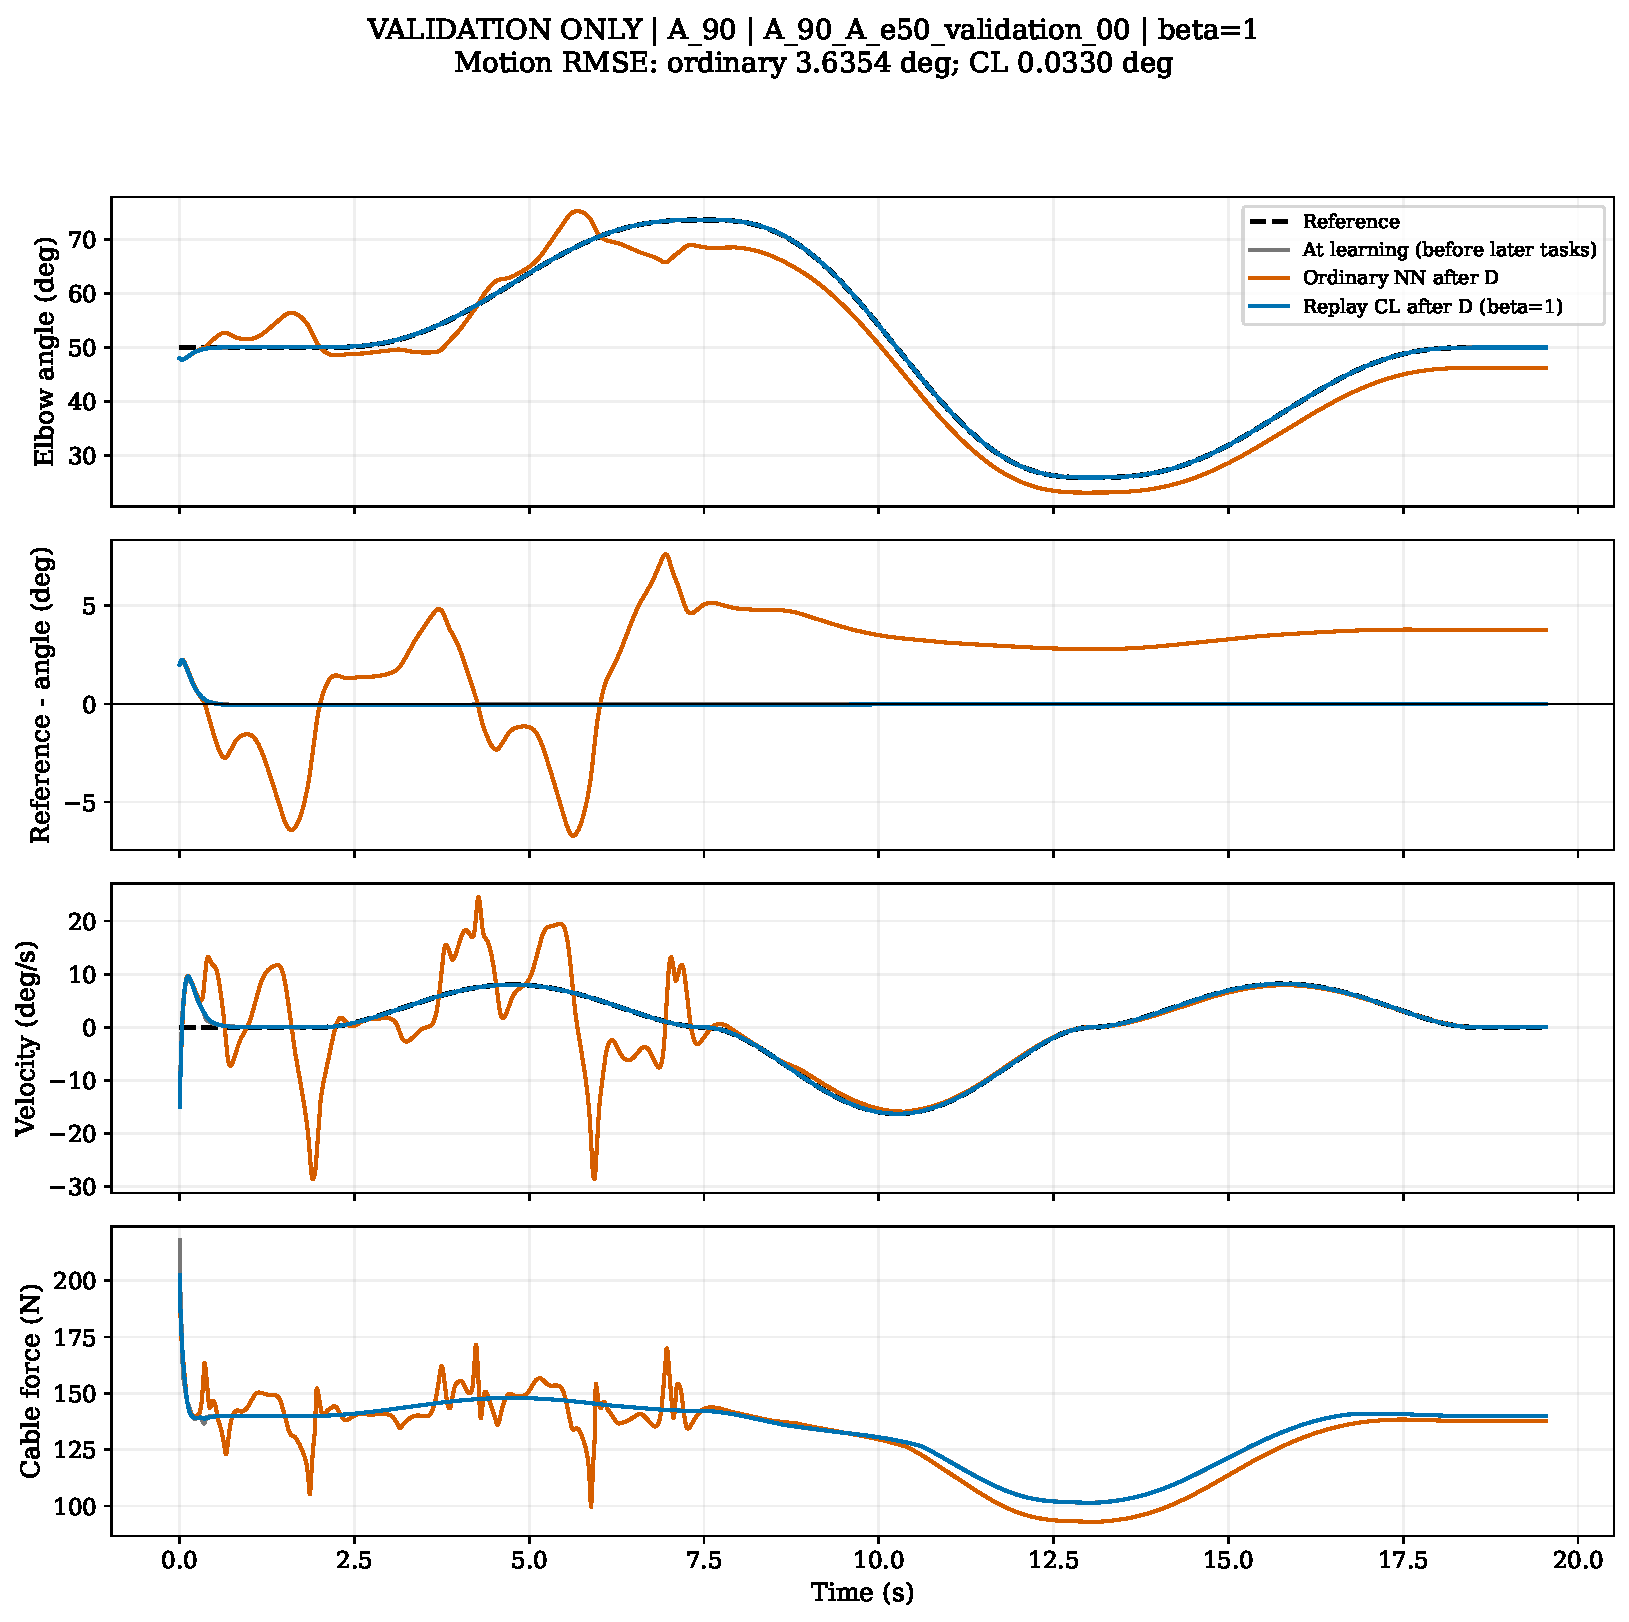
\includegraphics[width=\linewidth,height=.88\textheight,keepaspectratio]{figures/tracking/A_90/beta_1/A_90_A_e50_validation_00.pdf}
\clearpage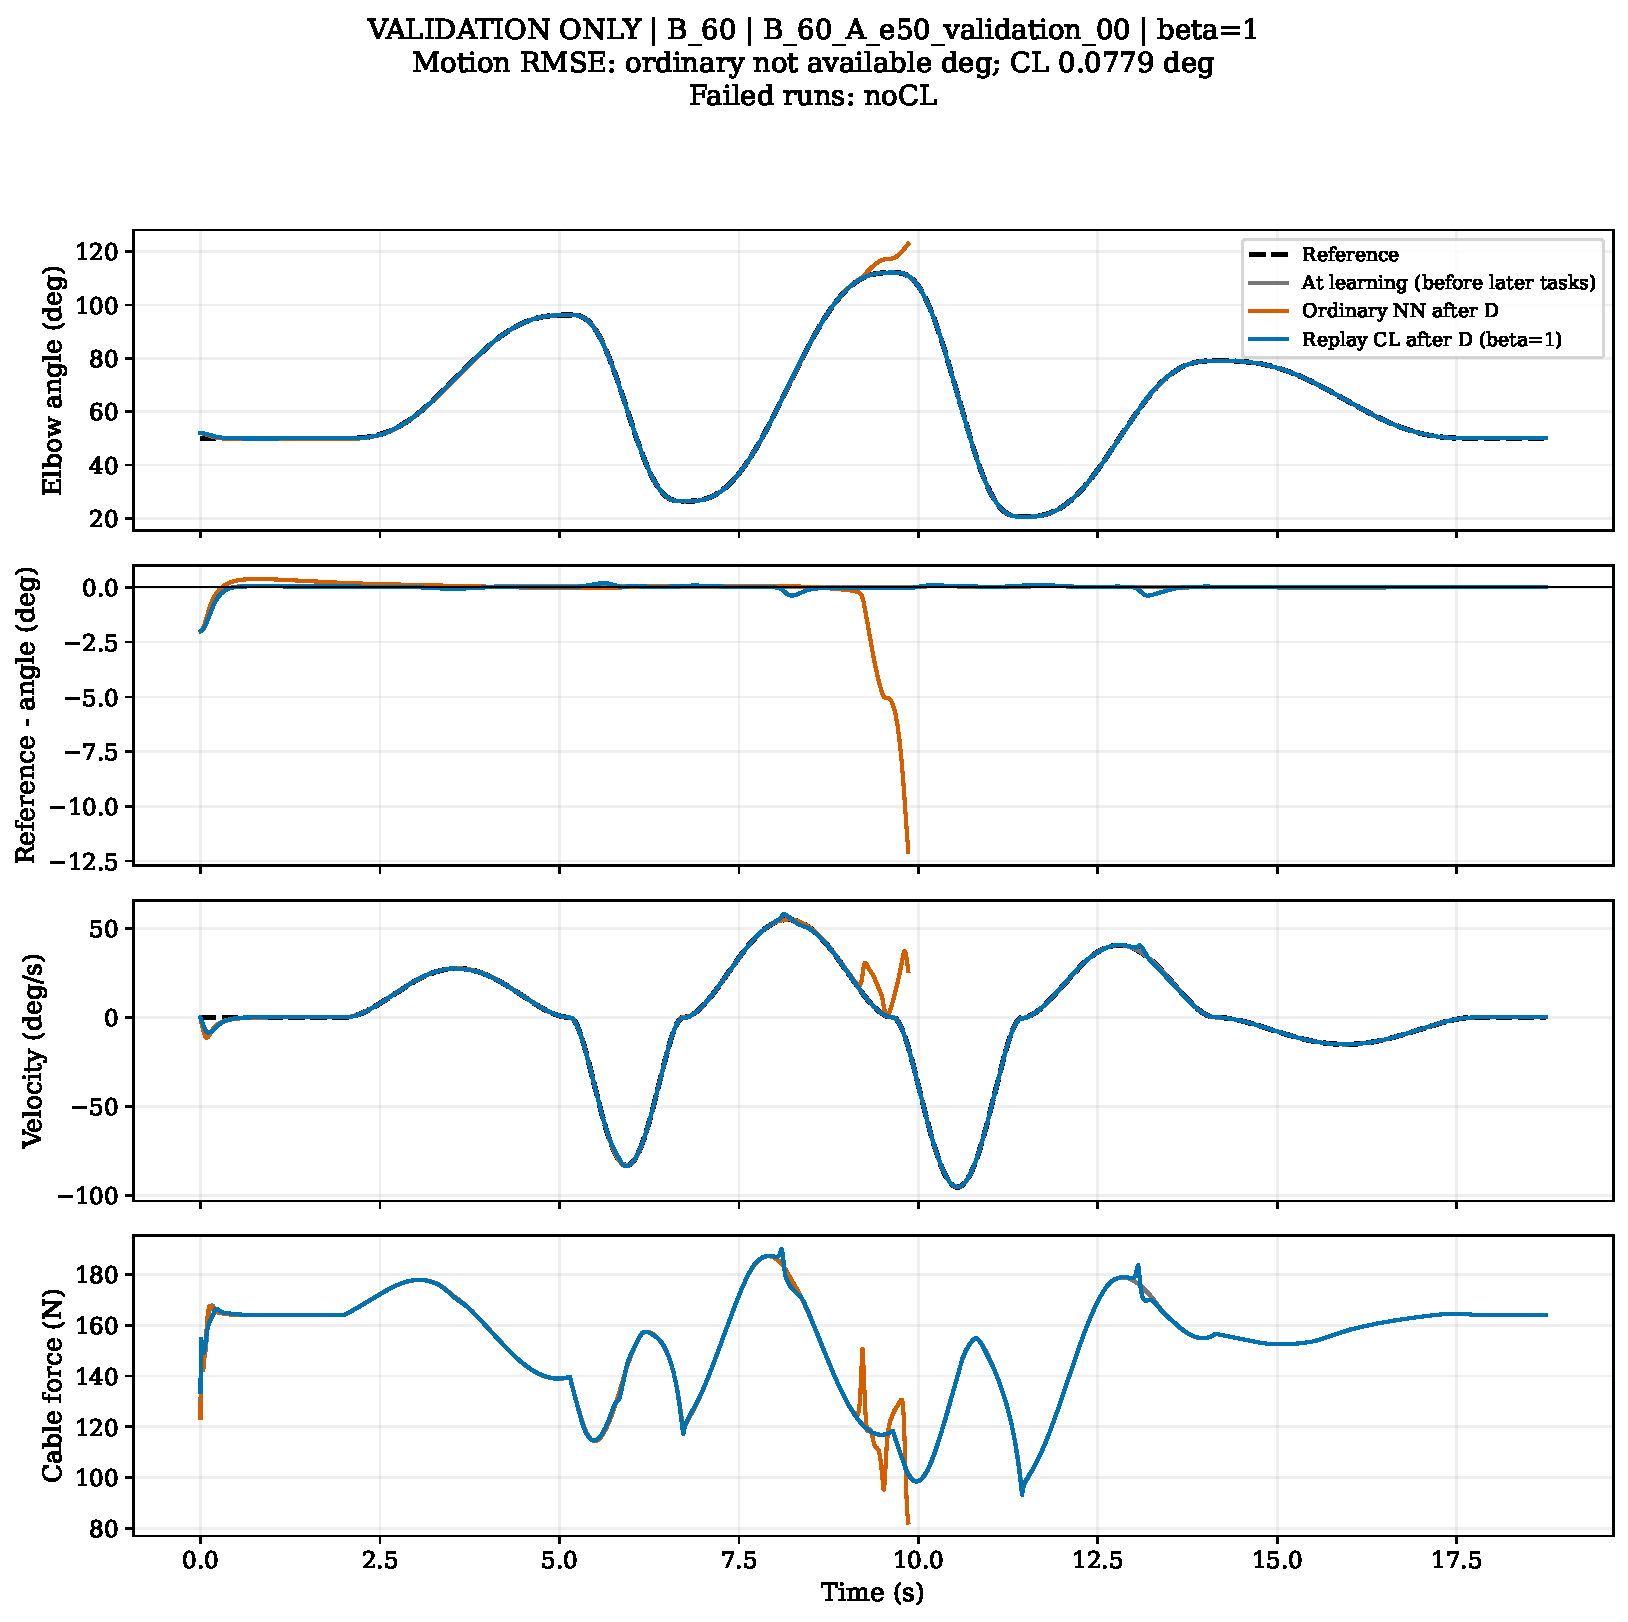
\includegraphics[width=\linewidth,height=.88\textheight,keepaspectratio]{figures/tracking/B_60/beta_1/B_60_A_e50_validation_00.pdf}
\clearpage\section*{Plasticity and eligibility}\small\begin{longtable}{llrrrl}\toprule Return & Beta/task & CL N & Ordinary N & Limit N & Gate\\\midrule
A\_90 & 1/B\_60 & 3.4287 & 1.5915 & 2.3873 & False\\
A\_90 & 1/C\_30 & 3.7336 & 1.4302 & 2.1453 & False\\
A\_90 & 1/D\_45 & 3.8977 & 1.7743 & 2.6614 & False\\
A\_90 & 4/B\_60 & 2.6826 & 1.5915 & 2.3873 & False\\
A\_90 & 4/C\_30 & 3.9504 & 1.4302 & 2.1453 & False\\
A\_90 & 4/D\_45 & 3.7196 & 1.7743 & 2.6614 & False\\
A\_90 & 16/B\_60 & 3.7308 & 1.5915 & 2.3873 & False\\
A\_90 & 16/C\_30 & 4.1590 & 1.4302 & 2.1453 & False\\
A\_90 & 16/D\_45 & 3.6391 & 1.7743 & 2.6614 & False\\
B\_60 & 1/C\_30 & 2.5706 & 1.4302 & 2.1453 & False\\
B\_60 & 1/D\_45 & 2.5956 & 1.7743 & 2.6614 & True\\
\bottomrule\end{longtable}\normalsize
Episode-level tracking errors, speed, force saturation, failures, and every individual return metric are saved in EPISODE\_METRICS.csv. Means in the summary use completed trials only; failed and total attempts are retained separately. The accuracy threshold is motion RMSE 0.5 degrees and motion peak 2 degrees. Full startup transients and full maximum errors are exported, even though the motion metric excludes the initial hold. Each comparison starts with a measured at-learning controller. If that initial controller fails the quality check, the report does not claim pure catastrophic forgetting.
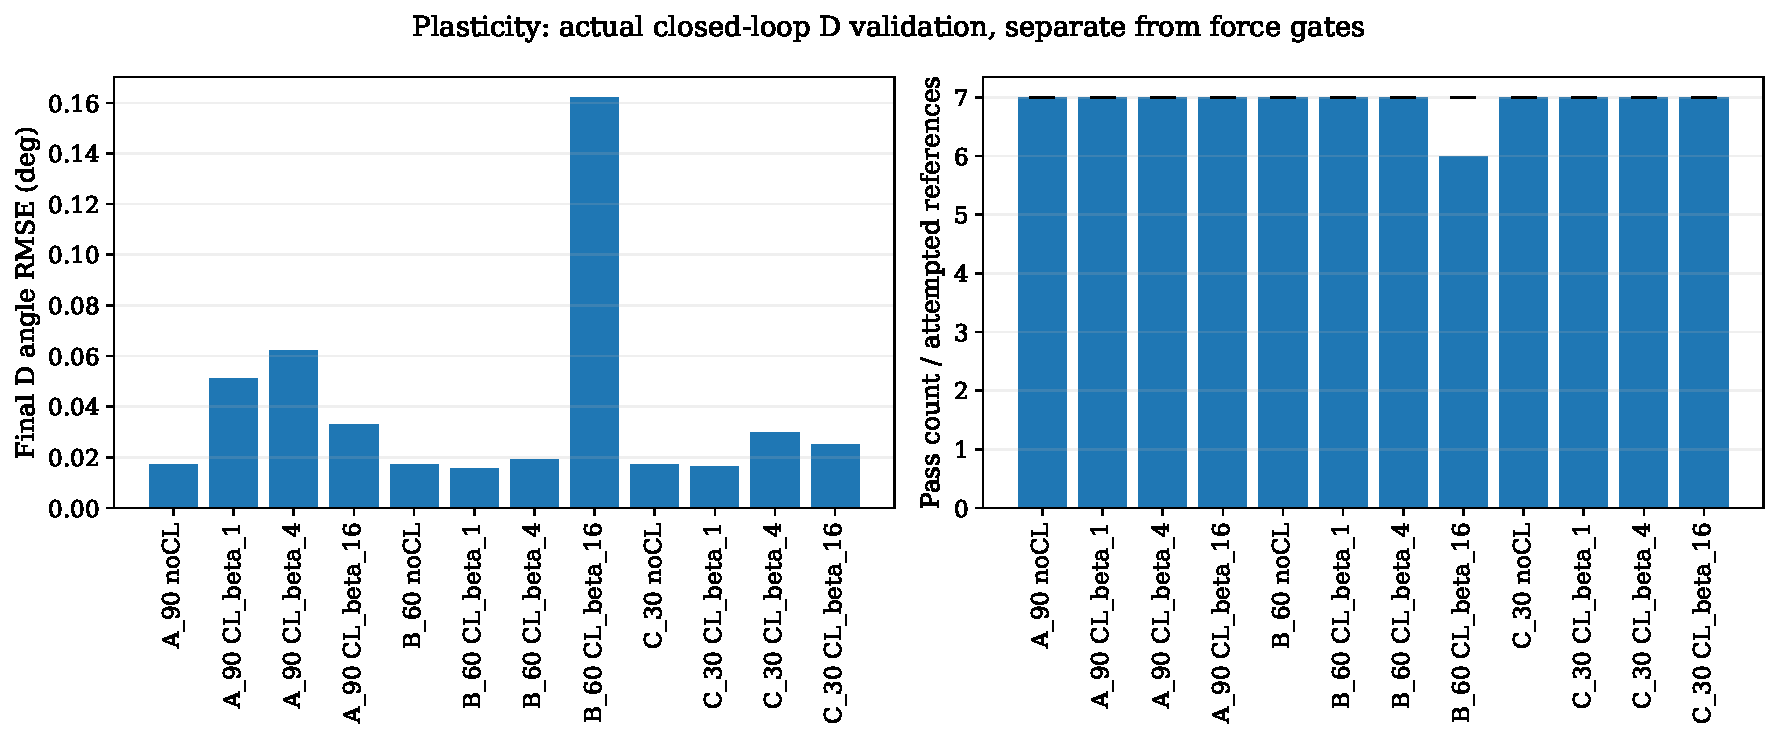
\includegraphics[width=\linewidth]{figures/summary/final_D_tracking.pdf}
\end{document}